\documentclass[10pt]{beamer}
\usepackage{anyfontsize}
\usepackage{minted}
\usepackage[T1]{fontenc}
% \usepackage{inconsolata}

\title[NIX]{NIX\\An HDF5-based data file format}
\author{Achilleas Koutsou}
\date{December 18, 2017}

\graphicspath{{./figures/}}

\begin{document}

\maketitle

\begin{frame}{G-Node}

    \begin{figure}
        
\includegraphics[width=0.4\textwidth]{g-node-logo.eps}
    \end{figure}

    \begin{itemize}
        \item Development and free distribution of tools for handling and neurophysiological data.
        \item All tools developed within the G-Node are open source and freely available.
        \item Main projects:
            \begin{itemize}
                \item {\color{red}NIX}:\ Manage data and metadata together in an open, versatile format.
                \item odML:\ Collect and manage all information about your experiment.
                \item GIN:\ Secure data storage, easy collaboration and publication.
            \end{itemize}
    \end{itemize}
\end{frame}

\begin{frame}{Data, results, and metadata}

    Data:
    \begin{itemize}
        \item Voltage traces, EEG recordings
        \item Subject location across time
        \item Subject preference to selection task
    \end{itemize}

    Analysis results:
    \begin{itemize}
        \item Spike times
        \item Total time the subject spent in an area
        \item Frequency of correct response over time
    \end{itemize}

    \pause{}

    Metadata:
    \begin{itemize}
        \item Recording equipment
        \item Subject age, gender, physical attributes
        \item Date, time, experimenter
    \end{itemize}

\end{frame}

\begin{frame}{Problems}

    The problem with (not necessarily) old datasets:
    \begin{itemize}
        \item Where did this dataset come from?
        \item When was it created?
        \item What were the simulation parameters when I generated these numbers?
        \item Who ran the experiment?
        \item What's the meaning of the second row of numbers?
    \end{itemize}
\end{frame}

\begin{frame}{NIX}{Features}

    Main features
    \begin{itemize}
        \item Open data format
        \item Store data, analysis results, and metadata conveniently in the same file
        \item Descriptive associations between data, analysis results and metadata
    \end{itemize}
\end{frame}

\begin{frame}{NIX}{Object hierarchy schema}
    \begin{figure}
        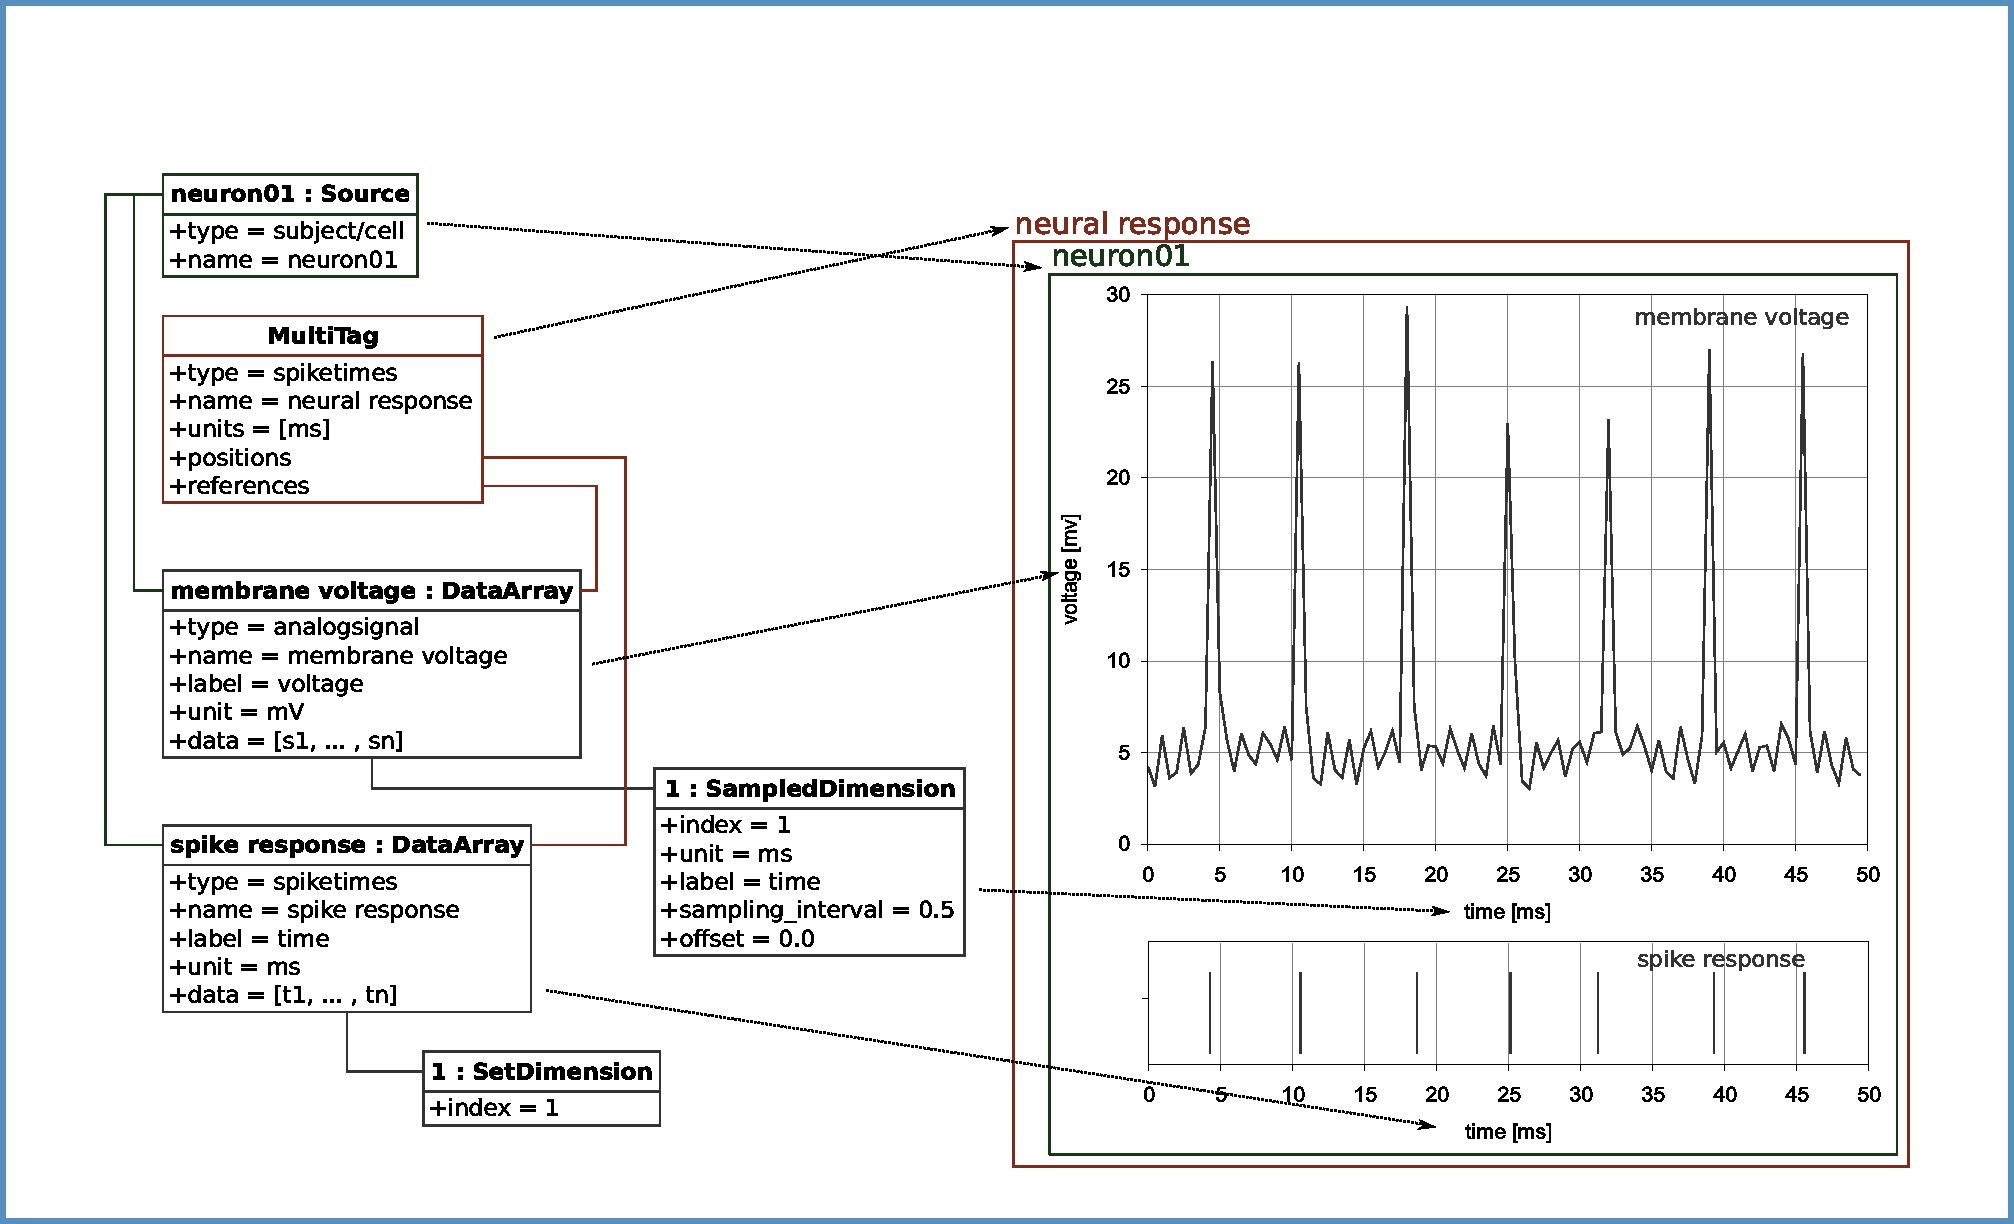
\includegraphics[width=\textwidth]{nix-model.pdf}
    \end{figure}
\end{frame}

\begin{frame}{NIX}{Libraries}
    Libraries available for multiple languages

    \begin{itemize}
        \item[C++] core library and reference implementation.
        \item[Python] bindings for core lib as well as complete reimplementation.
        \item[Matlab] bindings for core lib.
        \item[Java] bindings for core lib.
    \end{itemize}
    \begin{itemize}
        \item[Neo IO] allows interoperability with Neo, an API for organising electrophysiological data.
    \end{itemize}
\end{frame}

\begin{frame}{NIX}{Tooling}
    NixView --- Cross-platform GUI viewer

    \begin{columns}
        \begin{column}{0.5\textwidth}
            \begin{figure}
                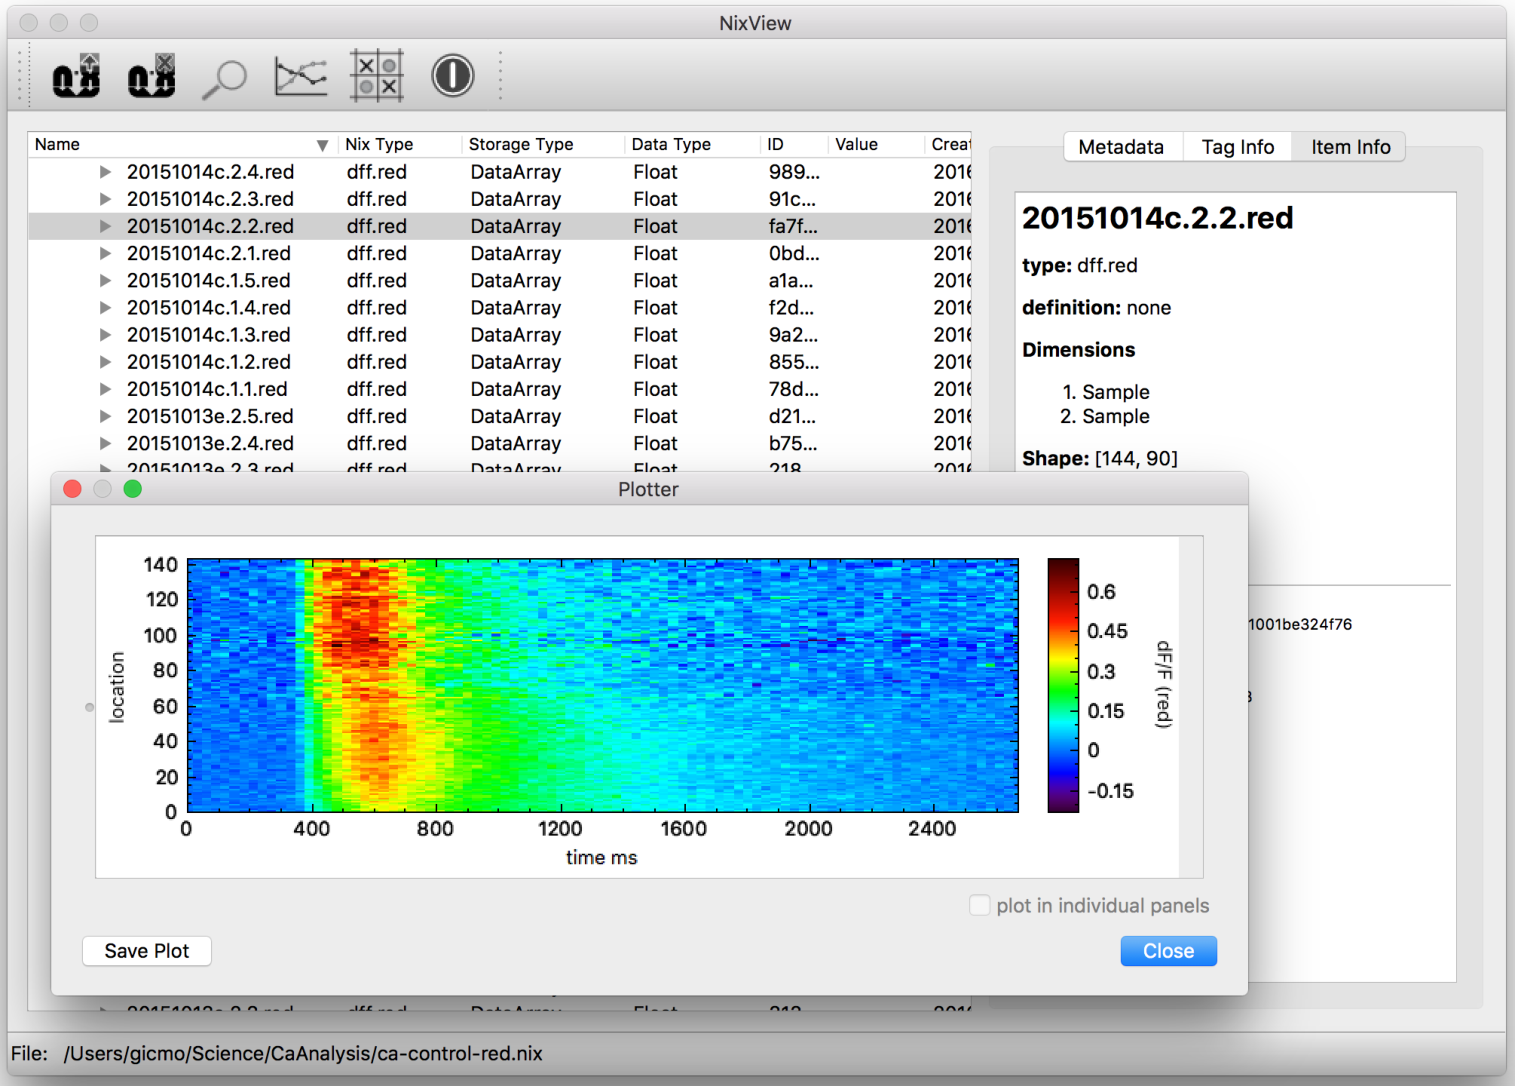
\includegraphics[width=\textwidth]{nixview.pdf}
            \end{figure}
        \end{column}
        \begin{column}{0.5\textwidth}
            \begin{itemize}
                \item Convenient exploration of data and metadata.
                \item Exports data to CSV.\
                \item Plotting of data.
            \end{itemize}
        \end{column}
    \end{columns}
\end{frame}

\begin{frame}[fragile]{NIX}{Python code}
    \inputminted[fontsize=\footnotesize,lastline=15]{python}{./code/nixify-data.py}
\end{frame}

\begin{frame}[fragile]{NIX}{Python code}
    \inputminted[fontsize=\footnotesize,firstline=17]{python}{./code/nixify-data.py}
\end{frame}

\begin{frame}[fragile]{NIX}{HDF5 structure}
    \inputminted[fontsize=\footnotesize]{shell}{./code/h5ls.out}
\end{frame}

\begin{frame}{NIX}{Data in NixView}
    \begin{figure}
        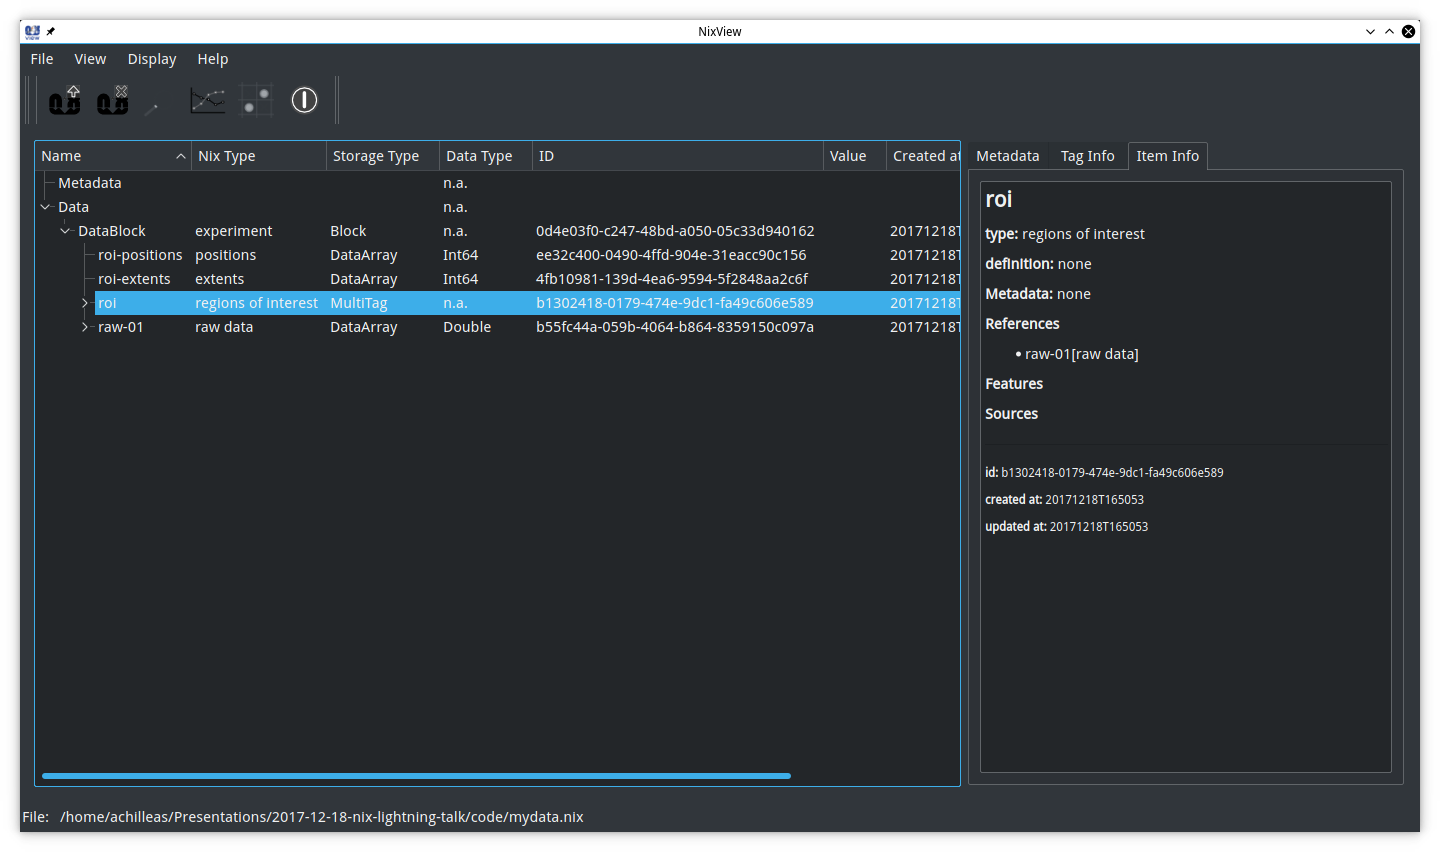
\includegraphics[width=\textwidth]{nixview-data.png}
    \end{figure}
\end{frame}

\begin{frame}{NIX}{Data in NixView}
    \begin{figure}
        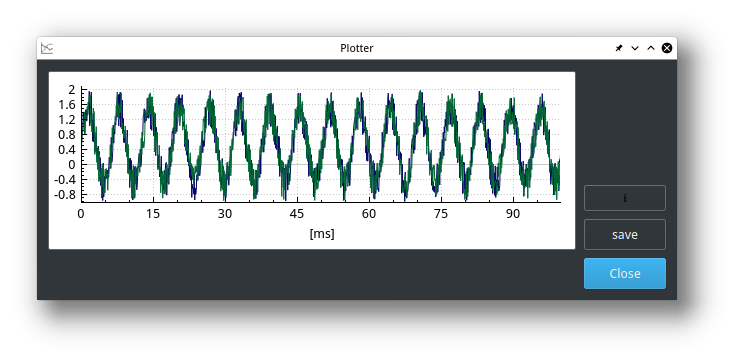
\includegraphics[width=\textwidth]{nixview-plot.png}
    \end{figure}
\end{frame}

\begin{frame}{NIX}{Resources}
    Resources

    \begin{itemize}
        \item NIX info and documentation: \url{https://github.com/G-Node/nix/wiki}
        \item NIX source: \url{https://github.com/G-Node/nix/}
        \item NIX Python source: \url{https://github.com/G-Node/nixpy/}
    \end{itemize}
\end{frame}

\end{document}
